%% 
%% Copyright 2007-2020 Elsevier Ltd
%% 
%% This file is part of the 'Elsarticle Bundle'.
%% ---------------------------------------------
%% 
%% It may be distributed under the conditions of the LaTeX Project Public
%% License, either version 1.2 of this license or (at your option) any
%% later version.  The latest version of this license is in
%%    http://www.latex-project.org/lppl.txt
%% and version 1.2 or later is part of all distributions of LaTeX
%% version 1999/12/01 or later.
%% 
%% The list of all files belonging to the 'Elsarticle Bundle' is
%% given in the file `manifest.txt'.
%% 

%% Template article for Elsevier's document class `elsarticle'
%% with numbered style bibliographic references
%% SP 2008/03/01
%%
%% 
%%
%% $Id: elsarticle-template-num.tex 190 2020-11-23 11:12:32Z rishi $
%%
%%
\documentclass[preprint,12pt]{elsarticle}

%% Use the option review to obtain double line spacing
%% \documentclass[authoryear,preprint,review,12pt]{elsarticle}

%% Use the options 1p,twocolumn; 3p; 3p,twocolumn; 5p; or 5p,twocolumn
%% for a journal layout:
%% \documentclass[final,1p,times]{elsarticle}
%% \documentclass[final,1p,times,twocolumn]{elsarticle}
%% \documentclass[final,3p,times]{elsarticle}
%% \documentclass[final,3p,times,twocolumn]{elsarticle}
%% \documentclass[final,5p,times]{elsarticle}
%% \documentclass[final,5p,times,twocolumn]{elsarticle}

%% For including figures, graphicx.sty has been loaded in
%% elsarticle.cls. If you prefer to use the old commands
%% please give \usepackage{epsfig}

%% The amssymb package provides various useful mathematical symbols
\usepackage{amssymb}
\usepackage{multirow}
\usepackage{lineno}
\usepackage[colorlinks,citecolor=black,linkcolor=black,urlcolor=black,bookmarks,bookmarksnumbered]{hyperref}
%% The amsthm package provides extended theorem environments
\usepackage{amsthm}
\usepackage{amsmath}

\newtheorem{theorem}{Theorem}[section]
\newtheorem{remark}[theorem]{Remark}
\newtheorem{lemma}{Lemma}[theorem]
\newtheorem{corollary}{Corollary}[theorem]
\newtheorem{definition}{Definition}[section]

%% The lineno packages adds line numbers. Start line numbering with
%% \begin{linenumbers}, end it with \end{linenumbers}. Or switch it on
%% for the whole article with \linenumbers.
%% \usepackage{lineno}

\journal{Energy}

\begin{document}
	
	%% TODO: UNCOMMENT THIS SECTION TO COMPILE ALSO INITIAL PART OF THE PAPER
	%
	%\begin{frontmatter}
		%
		%%% Title, authors and addresses
		%
		%%% use the tnoteref command within \title for footnotes;
		%%% use the tnotetext command for theassociated footnote;
		%%% use the fnref command within \author or \address for footnotes;
		%%% use the fntext command for theassociated footnote;
		%%% use the corref command within \author for corresponding author footnotes;
		%%% use the cortext command for theassociated footnote;
		%%% use the ead command for the email address,
		%%% and the form \ead[url] for the home page:
		%%% \title{Title\tnoteref{label1}}
		%%% \tnotetext[label1]{}
		%%% \author{Name\corref{cor1}\fnref{label2}}
		%%% \ead{email address}
		%%% \ead[url]{home page}
		%%% \fntext[label2]{}
		%%% \cortext[cor1]{}
		%%% \affiliation{organization={},
			%%%             addressline={},
			%%%             city={},
			%%%             postcode={},
			%%%             state={},
			%%%             country={}}
		%%% \fntext[label3]{}
		%
		%\title{Self-tunable approximated explicit MPC: Heat exchanger implementation and analysis}
		%%\title{Self-tunable approximated explicit MPC: Implementation on a heat exchanger with an asymmetric behavior}
		%
		%%% use optional labels to link authors explicitly to addresses:
		%%% \author[label1,label2]{}
		%%% \affiliation[label1]{organization={},
			%%%             addressline={},
			%%%             city={},
			%%%             postcode={},
			%%%             state={},
			%%%             country={}}
		%%%
		%%% \affiliation[label2]{organization={},
			%%%             addressline={},
			%%%             city={},
			%%%             postcode={},
			%%%             state={},
			%%%             country={}}
		%
		%\author{Lenka Galčíková}
		%\author{Petronela Belková}
		%\author{Juraj Oravec}
		%
		%\affiliation{organization={Slovak University of Technology in Bratislava, Faculty of Chemical and Food Technology, Institute of Information Engineering, Automation, and Mathematics,},%Department and Organization
			%            addressline={Radlinského 9}, 
			%            city={Bratislava},
			%            postcode={81237}, 
			%%            state={Slovakia},
			%            country={Slovakia}
			%}
		%
		%\begin{abstract}
			%%max 250 words!		
		
		The tunable approximated explicit model predictive control (MPC) comes with the benefits of real-time tunability without the necessity of solving the optimization problem online. This paper provides a novel self-tunable control policy that does not require any further tuning or interventions of the control engineer during operation. Based on the current operating conditions, the autonomous tuning parameter scales the control input using linear interpolation between the boundary optimal control actions. The adjustment of the tuning parameter depends on the current reference value, which makes this strategy suitable for reference tracking problems. Furthermore, a novel technique for scaling the tuning parameter is proposed. It provides to exploit different ranges of the tuning parameter assigned to specified operating conditions. The self-tunable explicit MPC was implemented on a laboratory heat exchanger with nonlinear and asymmetric behavior. To ensure offset-free reference tracking control, the built-in integrator was included in the explicit MPC design. The asymmetric behavior of the plant was compensated by tuning the controller's aggressiveness, as the negative or positive sign of reference change was considered in the tuning process. The designed self-tunable controller improved control performance by decreasing integral squared error, maximal overshoots/undershoots and settling time compared to the conventional control strategy based on a single (not tuned) controller. 
		%\end{abstract}
		%
		%%%Graphical abstract
		%\begin{graphicalabstract}
			%%\includegraphics{grabs}
			%\end{graphicalabstract}
		%
		%%%Research highlights
		%\begin{highlights}
			%% 3-5 highlights, every one should not exceed 85 characters including spaces
			%\item Self-tunable control technique does not need any intervention during control
			%\item Tuning based on the operating conditions compensates for the nonlinear plant behavior
			%\item Implementation of the proposed tuning method on a laboratory heat exchanger 
			%\item Control performance improved compared to utilizing only one explicit MPC
			%\end{highlights}
		%
		%\begin{keyword}
			%tunable explicit MPC \sep self-tunable technique \sep tuning parameter \sep heat exchanger \sep control performance
			%%% keywords here, in the form: keyword \sep keyword
			%
			%%% PACS codes here, in the form: \PACS code \sep code
			%
			%%% MSC codes here, in the form: \MSC code \sep code
			%%% or \MSC[2008] code \sep code (2000 is the default)
			%
			%\end{keyword}
		%
		%\end{frontmatter}
	
	%% \linenumbers
	
	%% main text
	\section{Introduction}
	\label{sec:introduction}
	
	
	%The main benefit in form of lower computational complexity in the control phase comes hand in hand with a non-negligible drawback. The size of the parametric solution may increase to the value that prevents its real-time implementation for two reasons: (i) the memory footprint is higher than the available memory size of the control unit, and (ii) the computational time associated with finding the optimal control action is higher than the available sample time for control action implementation. Although this control strategy has its challenges, it is still very beneficial for practical usage for its benefits. 
	
	The current crisis of energy resources emphasizes the long-term goal of achieving sustainable industrial production and optimal energy utilization. Moreover, minimizing the energy utilization directly reduces the corresponding CO$_{2}$ emissions. Therefore, sustainable industrial production is focused on the wide implementation of advanced control methods~\cite{MN20}. 
	
	The heat exchangers, in their numerous variants integrated into many industrial plants, represent energy-demanding plants. From the control viewpoint, the controller design taking into account the nonlinear and asymmetric behavior of the heat exchangers is a challenging task, see~\cite{RL20}. Although the conventional and widely-used proportional–integral–derivative (PID) controllers are robust and easy to tune, their control performance may not be sufficient when it comes to energy savings. Various extensions built above the well-tuned PID controller were developed to compensate for the nonlinear and asymmetric behavior, often affected by the additional impact of the uncertain parameters originated, e.g., in the fouling~\cite{MT19}. Such widely-used control strategies include, e.g., the robust control~\cite{DO15,WY18}, the gain-scheduling, multi-zone control, see~\cite{MF08}, and references therein.
	
	TODO: nepouzivat nasobne referencie ako [4,5] vyssie
	
	One of the promising control strategies addressing all these issues in an optimal way came with the formation and tuning of the model predictive control (MPC), e.g., see~\cite{Morari_MPC}. MPC provides optimal control input based on the minimization of a specified cost function while considering a model of the system. Compared to linear quadratic controllers (LQR)~\cite{LQR}, model predictive control also includes constraints on the control input or process variables~\cite{Maciejowski_MPC}, and additional saturation is not necessary. Moreover, as the optimization problem is solved in every control step, MPC represents a receding horizon control policy~\cite{receding_horizon}, having a significant benefit mainly in the terms of disturbance rejection. The model predictive control was intensively investigated in connection with heat exchangers. In~\cite{Vinaya_HE_MPC}, the authors developed a model predictive control for a shell and tube heat exchanger. In~\cite{Oravec_energy}, the control performance of the robust MPC implemented for a plate heat exchanger with soft constraints was analyzed. Four robust control strategies were presented and compared in~\cite{Oravec_HE_ATE}. A two-level control structure was applied on a heat exchanger network in~\cite{Gonzales_HE_MPC}, where the low level of control was ensured by MPC and the high level by a supervisory online optimizer.       
	
	The applicability of model predictive control expanded with the parametric solution of the MPC optimization problem, known as explicit MPC~\cite{Bemporad_automatica}. As the MPC optimization problem is pre-solved offline, it does not need to be solved in the online phase, i.e., in real-time control. Instead, a piece-wise affine (PWA) control law is evaluated to apply the optimal control action in each control step. The lower computational complexity makes the explicit MPC more suitable for practical industrial implementation. Nevertheless, the explicit MPC is not tunable in default as the conventional approach in~\cite{Bemporad_automatica} considers the penalty matrices with fixed structure and values.
	
	The possibility to tune the explicit MPC online came with the publishing of~\cite{Baric_tunable}. The tuning parameter penalizing the control inputs became a parameter, for which the optimal controller was precomputed. Nevertheless, the application was limited only to linear cost functions. To satisfy the demands for often-used quadratic cost functions, the approximated tunable explicit MPC was presented in~\cite{Klauco_tunable}. The technique is based on two explicit model predictive controllers which differ in the setup of one penalty matrix. The two explicit MPCs provide upper and lower boundary optimal controllers. Based on the evaluation of the two boundary control inputs, the tuned control input is calculated by linear interpolation. The follow-up work~\cite{Oravec_tunable} provided stability and recursive feasibility guarantees by proper choice of the terminal penalty matrix and terminal set constraint~\cite{Mayne_stability}. Moreover, the strategy in~\cite{Oravec_tunable} extends the tuning ability based on \textit{any} penalty matrix and not just the input penalty.
	
	The idea of approximated tunable MPC with neural networks is presented in~\cite{Kis_NN_MPC}. To ensure the tuning property, the penalty matrices were included in the training process. As a result, it was possible to tune the neural network-based controller online, while mimicking the nearly optimal MPC. In~\cite{Kis_NN_MPC_corrector}, the neural network-based tunable controller MPC was extended with a corrector which steered the controller such that the constraints on the manipulated and process variables were satisfied. 
	
	The paper~\cite{self_tunable} pushes the idea of tunable explicit MPC further and deals with the issues of practical industrial-oriented implementation. The procedure of the self-tunable controller technique is presented. The controller's aggressivity is tuned based on the difference between the reference value and the steady state corresponding to the model linearization point. Tuning based on the distance from the steady-state operating point represented a way how to compensate for the system's nonlinear behavior.
	
	This work directly extends our results presented in~\cite{self_tunable}, where the basic principles of the self-tunable approximated explicit MPC were introduced. In this paper, a novel method of self-tuning parameter setup is introduced. Compared to~\cite{self_tunable}, the self-tuning method is based on the size of the reference step change. Moreover, the idea of further scaling the tuning parameter is elaborated. The interval of the values of the self-tuning parameter is split at some certain value and each part of the interval corresponds to the specific operating conditions defined by the control engineer. In such a way, e.g., the system's asymmetric behavior is compensated. Finally, to investigate the benefits of the proposed approach, the proposed self-tuning control policy was implemented to control a laboratory-scaled counter-current plate heat exchanger. This work provides the control performance evaluation and analysis using the self-tunable controller compared to the boundary explicit MPCs.
	
	The paper is organized as follows. First, the theoretical backgrounds are presented in Section~\ref{sec:preliminaries}, where the explicit MPC, the approximated tunable explicit MPC, and existing self-tunable methods are briefly elaborated. Then, the novel proposed method of self-tunable procedure is explained in detail in Section~\ref{sec:methodology}. Finally, the experimental results of the self-tuning controller implementation on a heat exchanger are discussed in Section~\ref{sec:results}, followed by the main conclusions in Section~\ref{sec:conclusion}.
	
	\section{Theoretical backgrounds}
	% \section{Preliminaries}
	\label{sec:preliminaries}
	
	In this section, the theoretical backgrounds necessary for the proposed method are summarized. First, the explicit model predictive control is briefly recalled. Next, the tunable technique of the approximated explicit model predictive control is introduced. Finally, the ideas of a self-tunable technique of the approximated explicit MPC are presented.
	
	\subsection{Explicit model predictive control}
	\label{sec:eMPC}
	
	Explicit model predictive control~\cite{Bemporad_automatica} utilizes a parametric solution of the model predictive control introducing its application range towards the systems with fast dynamics. Moreover, the explicit solution enables providing rigorous analysis and certification of the closed-loop system stability, constraints satisfaction, etc. As the explicit solution is available, real-time solving of the optimization problem in every control step is omitted. As this work deals with industrial-oriented implementation, let us consider the optimization problem in the following form:
	\begin{subequations}
		\label{eq:mpc_problem}
		\begin{eqnarray}
			\label{eq:mpc_problem_cost}
			\min_{u_0,u_{1},\ldots,u_{N-1}} &~& \! \sum_{k=0}^{N-1} \! \left( (y_k-y_\mathrm{ref})^{\intercal} Q_\mathrm{y} (y_k-y_\mathrm{ref}) + u_{k}^{\intercal} R u_{k} + x_{\mathrm{I},k}^{\intercal} Q_\mathrm{x} x_{\mathrm{I},k} \right)  \\
			\label{eq:mpc_problem_prediction_model_x}
			\mathrm{s.t.\!:} &~& \widetilde{x}_{k+1} = \widetilde{A}\,\widetilde{x}_{k} + \widetilde{B}\,u_{k}, \\
			\label{eq:mpc_problem_prediction_model_y}
			&~& y_{k} = \widetilde{C}\,\widetilde{x}_{k}, \\
			\label{eq:mpc_problem_input_constraints}
			&~& u_{k} \in \mathcal{U}, \\
			\label{eq:mpc_problem_state_constraints}
			&~& y_{k} \in \mathcal{Y}, \\
			\label{eq:mpc_problem_initial_coindition}
			&~& \widetilde{x}_{0} = \theta, \\
			\label{eq:mpc_problem_k_range}
			&~& k = 0,1,\ldots, N-1,
		\end{eqnarray}
	\end{subequations}
	where $k$ denotes the step of the prediction horizon $N$. 
	%
	To obtain the offset-free control results, the built-in integrator was included in the state-space model, e.g., see~\cite{Ruscio_MPC_integral}. 
	The prediction model in Eq.~\eqref{eq:mpc_problem_prediction_model_x}--\eqref{eq:mpc_problem_prediction_model_y} has the form of augmented linear time-invariant (LTI) system for a given augmented state matrix $\widetilde{A} \in \mathbb{R}^{n_{\widetilde{\mathrm{x}}} \times n_{\widetilde{\mathrm{x}}}}$, augmented input matrix $\widetilde{B} \in \mathbb{R}^{n_{\widetilde{\mathrm{x}}} \times n_{\mathrm{u}}}$ and augmented output matrix $\widetilde{C} \in \mathbb{R}^{n_{\mathrm{y}} \times n_{\widetilde{\mathrm{x}}}}$. 
	%
	Variables $\widetilde{x} \in \mathbb{R}^{n_{\widetilde{\mathrm{x}}}}$, $u \in \mathbb{R}^{n_{\mathrm{u}}}$, $y \in \mathbb{R}^{n_{\mathrm{y}}}$ are vectors of corresponding augmented system states, control inputs, and system outputs, respectively. 
	%
	The sets $\mathcal{U} \subseteq \mathbb{R}^{n_{\mathrm{u}}}$, $\mathcal{Y} \subseteq \mathbb{R}^{n_{\mathrm{y}}}$ are convex polytopic sets of physical constraints on inputs and outputs, respectively. The penalty matrix $Q_\mathrm{y} \in \mathbb{R}^{n_{\mathrm{y}} \times n_{\mathrm{y}}}$ penalizes the squared control error, i.e., the deviation between the output and output reference value $y_\mathrm{ref}$. The matrix $R \in \mathbb{R}^{n_{\mathrm{u}} \times n_{\mathrm{u}}}$ penalizes the squarred value of control inputs. 
	%
	The value of integrator is also penalized in the cost function with the penalty matrix $Q_\mathrm{x} \in \mathbb{R}^{n_{\mathrm{y}} \times n_{\mathrm{y}}}$. 
	%
	The parameter $\theta \in \Theta$ in Eq.~\eqref{eq:mpc_problem_initial_coindition} represents the initial condition of the optimization problem for which it is parametrically pre-computed. 
	
	The augmented model of the controlled system with the built-in integrator in Eq.~\eqref{eq:mpc_problem_prediction_model_x}--\eqref{eq:mpc_problem_prediction_model_y} us rewritten as follows:
	\begin{subequations}
		\begin{eqnarray} 
			\label{eq:mpc_augmented_model_x} 
			\widetilde{x}_{k+1} &=& \begin{bmatrix} x_{k+1} \\ x_{\mathrm{I},k+1}\end{bmatrix} = \begin{bmatrix} A & \textit{0} \\ -T_\mathrm{s} C & I \end{bmatrix} \begin{bmatrix} x_{k} \\ x_{\mathrm{I},k} \end{bmatrix} + \begin{bmatrix} B \\ I \end{bmatrix} u_{k}, \\
			\label{eq:mpc_augmented_model_y}
			y_k &=& \begin{bmatrix} C & \textit{0} \end{bmatrix} \begin{bmatrix} x_{k} \\ x_{\mathrm{I},k} \end{bmatrix},
		\end{eqnarray}
	\end{subequations}
	where $x_{\mathrm{I}} \in \mathbb{R}^{n_{\mathrm{y}}}$ is the integral of the control error, $T_\mathrm{s}$ denotes the sampling time, and matrices $A$, $B$, $C$ are well-known the state-space matrices that form the augmented LTI model. As the consequence of this extension and penalization in the cost function in Eq.~\eqref{eq:mpc_problem_cost}, not only the control error is penalized, but also an integrated value, which leads to analogous offset-free reference tracking results as incorporating an integral part in PID controller.
	
	The parametric solution of the optimization problem of the quadratic programming (QP) in Eq.~\eqref{eq:mpc_problem}, leads to the explicit solution in the form of piecewise affine PWA control law defined above the domain consisting of $r$ critical regions:
	\begin{eqnarray}
		\label{eq:PWA_control_law}
		u(\theta) = \left\{ 
		\begin{matrix}
			F_{1} \, \theta + g_{1} & \mathrm{if} & \quad \theta \in \mathcal{R}_1, \\
			F_{2} \, \theta + g_{2} & \mathrm{else}\,\,\mathrm{if} &\quad \theta \in \mathcal{R}_2, \\
			\vdots & \\
			F_{r} \, \theta + g_{r} & \mathrm{else}\,\,\mathrm{if} & \quad \theta \in \mathcal{R}_{r}, \\
		\end{matrix}
		\right.
	\end{eqnarray}
	where $F_{i} \in \mathbb{R}^{n_{\mathrm{u}} \times n_{\mathrm{x}}}$ and $g_{i}  \in \mathbb{R}^{n_{\mathrm{u}}}$ respectively are the slope and affine section of the corresponding control law. The PWA function defined in Eq.~\eqref{eq:PWA_control_law} is stored and recalled in the online phase, i.e., during the real-time control. Based on identifying the specific critical region $\mathcal{R}_{i}$, where the parameter $\theta$ belongs, the optimal control input is calculated based on the associated control law in Eq.~\eqref{eq:PWA_control_law}.
	
	Note, many other formulations of the optimization problems for the explicit MPC design, were mainly in the terms of the definition of the cost functions in Eq.~\eqref{eq:mpc_problem_cost}. Also, the incremental (velocity) formulation of the state-space model is common, but leads to further extension of the vector of parameters $\theta$, and therefore also the complexity of the explicit MPC controller increases. Another option for offset-free tracking is introducing disturbance modeling and estimation. For such an overview see e.g.~\cite{Klauco_mpc} 

	
	\subsection{Tunable explicit model predictive control}
	\label{sec:tunable}
	
	The aggressivity of the controller and the whole nature of the control is influenced by appropriate fine-tuning of the penalty matrices in the optimization problem in Eq.~\eqref{eq:mpc_problem}. When the multi-parametric QP (mp-QP) problem is precomputed offline to obtain the corresponding parametric solution, it is not possible to tune the controller afterward without trading off a significant increase in the controller complexity or the performance loss. As the operating conditions and requirements of controller setup may differ throughout the control, the ability to adjust the controller's aggressivity can be very beneficial.
	
	The idea of approximated tunable explicit MPC comes from the work ~\cite{Klauco_tunable}, where the control action is calculated based on linear interpolation between two boundary control actions. These control actions result from evaluating two boundary explicit MPCs. The boundary explicit controllers have the same structure and setup, except for one of the penalty matrices -- the tuned one. The boundary penalty matrices are diagonal square matrices such that $\lambda_{i,\mathrm{L}} \le \lambda_{i,\mathrm{U}}$, $\forall i = 1,\dots,s$, where $\lambda$ denotes the vector of eigenvalues of the penalty matrix, $s$ is the rank of the tuned penalty matrix, and $L$, $U$ denote the lower and upper boundary setup respectively.
	
	Let us consider the penalty matrices in the cost function in Eq.~\eqref{eq:mpc_problem_cost}. The penalty matrices are scaled in the following way:
	\begin{subequations}
		\label{eq:tunable_matrices}
		\begin{eqnarray}
			\label{eq:tunable_R}
			&~& R(k) = (1-\rho(k)) \, R_\mathrm{L} + \rho(k) \, R_\mathrm{U}, \\
			\label{eq:tunable_Qx}
			&~& Q_\mathrm{x}(k) = (1-\rho(k)) \, Q_\mathrm{x,L} + \rho(k) \, Q_\mathrm{x,U}, \\
			\label{eq:tunable_Qy}
			&~& Q_\mathrm{y}(k) = (1-\rho(k)) \, Q_\mathrm{y,L} + \rho(k) \, Q_\mathrm{y,U},
		\end{eqnarray}
	\end{subequations}
	where $\rho$ represents the tuning parameter such that $0 \le \rho \le 1$ holds. Based on the rules in Eq.~\eqref{eq:tunable_matrices}, it is possible to choose online any controller setup from the lower to the upper boundary of the tuned matrix. From the implementation point of view, it is preferred to tune just a single penalty matrix, i.e., to store only two controllers corresponding to the boundary values of the selected penalty matrix. To determine which penalty matrix in Eq.~\eqref{eq:tunable_matrices} should be tuned, it is suggested to judge the control performance subject to the specific system and systematically tune all of the penalty matrices.
	
	When the tuning parameter $\rho$ is determined based on the current control conditions, the approximated optimal control action is evaluated using the two optimal controllers. Based on the boundary control actions, the interpolated, i.e., tuned control action is calculated using the convex combination:
	%\begin{subequations}
		\begin{eqnarray}
			\label{eq:tunable_u}
			u(k) = (1-\rho(k)) \, u_\mathrm{L}(k) + \rho(k) \, u_\mathrm{U}(k),
		\end{eqnarray}
		%\end{subequations}
	where $u_\mathrm{L}$ and $u_\mathrm{U}$ denote the optimal control actions from the lower and upper boundary controller respectively. The online tuning of the controller online comes with the cost of storing and evaluating two explicit controllers. Nevertheless, the ability to tune the controller may be more important in many practical applications.
	
	The concept of explicit MPC tuning is applicable to a wide class of MPC design formulations, based on the current specific needs. Without loss of generality, hereafter, let us consider the penalty matrices of the cost function in Eq.~\eqref{eq:mpc_problem_cost}, as it is necessary to satisfy offset-free reference tracking.
	
	\begin{remark}
		If the asymptotic stability and recursive feasibility guarantees are required, the reader is referred to follow the instructions from \cite{Oravec_tunable}. In order to satisfy these requirements, the study introduces a procedure for computing the common terminal penalty and terminal set for the two boundary controllers. 
	\end{remark}

	\begin{remark}
		Not only Eq.~\eqref{eq:tunable_u} needs to be chosen for interpolation of the control input. Another way of tuning the control input can be using some nonlinear relation for the interpolation. 
	\end{remark}


	
	\subsection{Self-tunable explicit model predictive control}
	\label{sec:self_tunable}	
	The advantage of a tunable controller brings a question of how to design the logic of setting the tuning parameter $\rho$. In this section, the idea of online self-tuning is summarized~\cite{self_tunable}. The concept of self-tuning provides the possibility to adjust the aggressiveness of the controller without the necessity to intervene and tune the penalty matrices during control. 
	
	The need for real-time controller tuning often arises from tracking a time-varying piece-wise constant (PWC) reference. The work~\cite{self_tunable} focuses on adjusting the penalty matrix when the reference value is changed. The further the reference value is from the steady state, the more aggressively the controller is tuned. The idea behind the suggested scaling lies in compensation for the nonlinear behavior of the system.  
	
	Consider a single-input and single-output (SISO) system or a multiple-inputs and multiple-outputs (MIMO) system with completely decoupled pairs of the control inputs and the system outputs. 
	Then, the procedure of tuning the controller is based on evaluating the different operating points between the current value of the reference and the system steady-state value. This deviation is considered to scale the value of control action. First, the maximal admissible absolute value of the reference is defined. Analogous to the reference trajectory preview concept of MPC design, this value can be determined based on the general knowledge of the expected future reference values. Another suggestion is to fit the maximal deviation $d_{\max}$ based on the constraints on system outputs: 
	\begin{eqnarray}
		\label{eq:d_max}
		d_{\max} = \max(\vert y_{\min} \vert, y_{\max}),
	\end{eqnarray}
	where $y_{\min}$ and $y_{\max}$ are respectively lower and upper bound on the output variable in the deviation form, i.e., zero corresponds to the system steady-state value. Using the information about the maximal possible deviation $d_{\max}$, the tuning parameter $\rho$ can be calculated as the ratio between the current reference value and the maximal deviation:  
	\begin{eqnarray}
		\label{eq:rho_self_tunable}
		\rho = \frac{\vert y_{\mathrm{ref}(k)} \vert}{d_{\max}}.
	\end{eqnarray}
	
	Based on Eq.~\eqref{eq:rho_self_tunable}, the property $0 \le \rho \le 1$ holds, as $\vert y_{\mathrm{ref}} \vert \le d_{\max}$. As a consequence, the parameter $\rho$ represents a way how to normalize the deviation from the steady-state value and is exploited to scale the penalty matrix or, implicitly, to scale the aggressiveness of the control action. 
	
	When considering tuning the control action based on Eq.~\eqref{eq:tunable_u}, a higher value of tuning parameter $\rho$ leads to approaching the upper boundary controller and vice versa. When tuning, e.g., the matrix $Q_\mathrm{y}$ penalizing the control error, a higher ratio $\rho$ would lead to more aggressive control actions. When operating with the reference value close to the system steady-state value, the parameter $\rho$ decreases and the control profiles become sluggish.
	
	\begin{remark}
		In general, the parameter $d_{\max}$ is a vector, as it depends on the size of the system outputs. If $d_{\max}$ is scalar, the parameter $\rho$ is scalar as well and can be directly utilized to scale the control action. If multiple outputs are controlled, it is suggested to calculate the tuning parameter based on the maximal ratio:
		\begin{eqnarray}
			\label{eq:rho_max}
			\rho(k) = \max \left( \frac{\vert y_{\mathrm{ref}}(k) \vert}{d_{\max}} \right).
		\end{eqnarray}
	\end{remark}
	
	Note, the relations in Eq.~\eqref{eq:rho_self_tunable} and Eq.~\eqref{eq:rho_max} operate with the absolute value of the reference. It is not taken into account, whether the reference change was positive or negative with respect to the system steady-state value placed in the origin, i.e., whether it changed upwards or downwards. As many plants have asymmetric behavior, the positivity or negativity of the reference change could be considered in the controller tuning to improve the control performance.
	
	
	\section{Methodology}
	\label{sec:methodology}
	This section extends the ideas of self-tunable explicit MPC in order to improve control performance. First, a different way of tuning parameter calculation is introduced. Furthermore, an extended self-tunable technique is presented to scale the tuning parameter for industrial-oriented applications, when it is beneficial to exploit a specific range of the tuning parameter in different operating conditions. 
	
	
	\subsection{Tuning parameter based on the size of reference change}
	\label{sec:self_tunable_delta_ref}
	The approach of self-tunable explicit MPC in~\cite{self_tunable} suggested tuning based on the current reference value distance from the steady state. The aim is to compensate for the nonlinear behavior of a system when using a simple linear prediction model. This work provides also another useful way of the real-time evaluation of the tuning parameter $\rho$ based on the size of reference change. When different sizes of reference step changes are made and the behavior of the closed-loop system is varying, it can be beneficial to include the size of the reference step change in the tuning procedure.
	
	In this approach, the aggressivity is adjusted based on the ratio between the reference step change and the maximal reference step change that can be realized during the control operation:
	\begin{eqnarray}
		\label{eq:rho_delta_ref}
		\rho(k) = \frac{\vert \Delta_{\mathrm{ref}}(k) \vert}{\Delta_{\max}},
	\end{eqnarray} 
	where $\Delta_{\mathrm{ref}}(k) = y_{\mathrm{ref}}(k) - y_{\mathrm{ref}}(k-1)$ is the size of the reference step change. The denominator of Eq.~\eqref{eq:rho_delta_ref} is changed as well. In contrast to the maximal deviation from the steady state in Section~\ref{sec:self_tunable}, this approach introduces $\Delta_{\max}$ as the maximal possible reference step change. Analogously to the original approach, the maximal reference step can be set based on the general knowledge of the expected future reference values, i.e., $\Delta_{\max} = \Vert \Delta_{\mathrm{ref}}(k) \Vert_{\infty}, \forall k \ge 0 $. 
	Another option is to exploit the information about the system constraints and set the parameter $\Delta_{\max}$ according to Eq.~\eqref{eq:d_max}. 
	
	Note, only the absolute value of $\Delta_{\mathrm{ref}}$ and $\Delta_{\max}$ are considered in this procedure to ensure $\rho \ge 0$. 
	
	\begin{remark}
		The tuning parameter $\rho$ should be updated only when the reference changes. Updating the tuning parameter in the control steps when $\Delta_{\mathrm{ref}} = 0$ would lead to using tuning parameter $\rho$ with zero value, i.e., the control input would correspond to one boundary controller and would not be scaled.
	\end{remark}
	
	
	\subsection{Self-tunable technique for systems with asymmetric behavior}
	\label{sec:self_tunable_rho_scaling}
	
	This paper provides a further extension of the self-tuning method proposed in~\cite{self_tunable}. The suggested technique of tuning is suitable, e.g., for systems with asymmetric behavior, but can be used in any application, where ``simple'' tuning in the whole range of tuning parameter $\rho$ is not sufficient.
	
	The proposed self-tuning method is based on splitting the interval of the tuning parameter $\rho$ in order to utilize different parts of the interval in different operating conditions. Instead of the original value of tuning parameter $\rho$, the adjusted tuning parameter $\widetilde{\rho}$ is then utilized to scale the control input according to Eq.~\eqref{eq:tunable_u}.
	
	%% TODO: DEF RULE/CONDITION GAMMA
	\begin{definition}[Decision function]
		\label{def:gamma}
		For a given interval of tuning parameter $\rho$, $0 \leq \rho \leq 1$, let $\rho_{\mathrm{s}}$, $0 < \rho_{\mathrm{s}} < 1$ be a boundary value splitting the interval into two parts. Let $\gamma: \mathbb{R} \rightarrow \mathbb{R}$ be an arbitrary function such that $0 \leq \gamma \leq 1$ holds. Then the decision function $\gamma$ is constructed to assign its value either $\gamma \leq \rho_{\mathrm{s}}$ or $\gamma \ge \rho_{\mathrm{s}}$.
	\end{definition}
	Various decision functions $\gamma$ can be considered. In this work, the decision functions according to Eq.~\eqref{eq:rho_max} and Eq.~\eqref{eq:rho_delta_ref} are considered, while Eq.~\eqref{eq:rho_delta_ref} was implemented in the experimental case study.
	
	\begin{definition}[Scaling tuning parameter]
		\label{def:rho_tilde}
		Given the value of tuning parameter $\rho$, $0 \leq \rho \leq 1$, in control law~\eqref{eq:PWA_control_law}, the splitting value of the tuning parameter interval $\rho_{\mathrm{s}}$, $0 < \rho_{\mathrm{s}} < 1$, and the value of the decision function $\gamma$, $0 < \gamma < 1$. Then the scaling tuning parameter $\widetilde{\rho}$ is given by:		
		\begin{eqnarray}
			\label{eq:rho_tilde_def}
			\widetilde{\rho} = \left\{ 
			\begin{matrix}
				\rho \, \rho_{\mathrm{s}} & \mathrm{if} & \quad \gamma \in \langle 0, \rho_{\mathrm{s}} \rangle , \\
				\rho \, (1-\rho_{\mathrm{s}}) + \rho_{\mathrm{s}}, & \mathrm{else}\,\,\mathrm{if} &\quad \gamma \in \langle \rho_{\mathrm{s}}, 1 \rangle.
			\end{matrix}
			\right.
		\end{eqnarray}
		\end{definition}

%\begin{definition}
%		If the tuning parameter is scaled in the first part of the interval, i.e., $\langle 0, \rho_{\mathrm{s}} \rangle$, where $\rho_{\mathrm{s}}$ is the splitting value of the tuning parameter interval, the following relation is used to adjust the tuning parameter:
%		\begin{eqnarray}
%			\label{eq:rho_up}
%			\widetilde{\rho} = \rho_{\mathrm{s}} \rho.
%		\end{eqnarray}
%		$\widetilde{\rho}$ such that $0 \leq \widetilde{\rho} \leq 1$ 
%\end{definition}

%	\begin{definition}
%	Given the current parameter value $\rho$. If the tuning parameter is scaled in the second part of the interval, i.e., $\langle \rho_{\mathrm{s}}, 1 \rangle$, the following relation is used to adjust the tuning parameter:
%	\begin{eqnarray}
%		\label{eq:rho_down}
%		\widetilde{\rho} = (1-\rho_{\mathrm{s}}) \rho + \rho_{\mathrm{s}}.
%	\end{eqnarray}
%	\end{definition}
	
	\begin{remark}
	\label{rem:rho_tilde}		
		The introduction of splitting the scaling tuning parameter $\widetilde{\rho}$ into the tuning intervals in~\eqref{eq:rho_tilde_def} is not limited only to two intervals. If the nature of the controlled plant would benefit from splitting the operating range into more intervals, e.g., when the plant operates in the multiple steady-states values, then these intervals are simply determined by the corresponding values of $\rho_{\mathrm{s}, i}$ for each part of the interval. Next, the tuning rules in~\eqref{eq:rho_tilde_def} are adopted in an analogous way.
	\end{remark}
	
	The following outcomes result from Eq.~\eqref{eq:rho_tilde_def}. 
	%	\begin{corollary}
	% The following outcomes result from Eq.~\eqref{eq:rho_up}. If $\rho=0$, then $\widetilde{\rho} = 0$. When considering the other extreme, i.e., $\rho=1$, then $\widetilde{\rho} = \rho_{\mathrm{s}}$. In such a way, the parameter $\rho$ can be scaled in the first part of the interval up to the splitting value. Note, as the relation in Eq.~\eqref{eq:rho_up} is linear and $0 \le \rho \le 1$ holds, for $\widetilde{\rho}$ it is impossible to acquire other values than in the given interval of parameter $\rho$.		
	%	\end{corollary}
	%
	%	\begin{corollary}
	%		The following outcomes result from Eq.~\eqref{eq:rho_down}. When $\rho=0$, $\widetilde{\rho} = \rho_{\mathrm{s}}$. When considering the other extreme, i.e., $\rho=1$, then $\widetilde{\rho} = 1$. In such a way, the parameter $\rho$ can be scaled in the second part of the interval from the splitting value up to 1. Note, as the relation in Eq.~\eqref{eq:rho_down} is linear and $0 \le \rho \le 1$ holds, for $\widetilde{\rho}$ it is impossible to acquire other values than in the given interval of parameter $\rho$.
	%	\end{corollary}
	\begin{lemma}
		\label{lem:PWA_control_law_interval}
		Given control law in~\eqref{eq:PWA_control_law}, its approximation given by the convex combination in~\eqref{eq:tunable_u}, and given scaling tuning parameter $\widetilde{\rho}$ according Definition~\ref{def:rho_tilde}. Then the control law  approximated into the form:
		\begin{eqnarray}
			\label{eq:PWA_control_law_interval}
			u(k) = (1-\widetilde{\rho}(k)) \, u_\mathrm{L}(k) + \widetilde{\rho}(k) \, u_\mathrm{U}(k),
		\end{eqnarray}
		preserves the closed-loop system stability and recursive feasibility of the original control law in~\eqref{eq:PWA_control_law}.
	\end{lemma}

	\begin{proof}
		\label{proof:rho_tilde}
		It has been proven~\cite{Oravec_tunable} that for the asymptotic stable and recursive feasible pair of control inputs $(u_{\mathrm{L}}, u_{\mathrm{U}})$, the approximated control law in~\eqref{eq:PWA_control_law} preserves these properties for any $\rho$ satisfying $0 \leq \rho \leq 1$, see Theorem~3.6 in~\cite{Oravec_tunable}. 
		% 
		It remains to prove that for any value of the scaling tuning parameter $\widetilde{\rho}$ according to the Definition~\ref{def:rho_tilde} the same results hold. 
		The rest of the proof of Lemma~\ref{lem:PWA_control_law_interval} consists of two parts corresponding to each particular rule in~\eqref{eq:rho_tilde_def}. 
		\\
		First, it is proved that the Lemma~\ref{lem:PWA_control_law_interval} holds for any $\gamma \leq \rho_{\mathrm{s}}$. Substituting a lower bound $\rho=0$ into~\eqref{eq:rho_tilde_def} leads to
		$\widetilde{\rho} = 0$. 
		For the upper bound value of $\rho=1$, from~\eqref{eq:rho_tilde_def} holds $\widetilde{\rho} = \rho_{\mathrm{s}} < 1$. Next, for any value $0 < \rho < 1$ evaluation of the linear rule in~\eqref{eq:rho_tilde_def} leads to the convex combination, i.e., $0 < \widetilde{\rho} < \rho_{\mathrm{s}} $ holds. 
		Therefore, any value of $\widetilde{\rho}$ satisfies $0 \leq \widetilde{\rho} \leq \rho_{\mathrm{s}} < 1$. As the consequence, according to the Theorem~3.6 in~\cite{Oravec_tunable}, the asymptotic stability and recursive feasibility of the control law in~\eqref{eq:PWA_control_law_interval} are preserved. 
		\\
		Secondly, it is proved that the Lemma~\ref{lem:PWA_control_law_interval} holds also for any $\gamma \geq \rho_{\mathrm{s}}$. Substituting a lower bound $\rho=0$ into~\eqref{eq:rho_tilde_def} leads to
		$\widetilde{\rho} = \rho_{\mathrm{s}}$. 
		For the upper bound value of $\rho=1$, from~\eqref{eq:rho_tilde_def} holds $\widetilde{\rho} = 1$. Next, for any value $0 < \rho < 1$ evaluation of the linear rule in~\eqref{eq:rho_tilde_def} leads to the convex combination, i.e., $\rho_{\mathrm{s}} < \widetilde{\rho} < 1 $ holds. 
		Therefore, any value of $\widetilde{\rho}$ satisfies $\rho_{\mathrm{s}} \leq \widetilde{\rho} \leq 1$. As the consequence, according to the Theorem~3.6 in~\cite{Oravec_tunable}, the asymptotic stability and recursive feasibility of the control law in~\eqref{eq:PWA_control_law_interval} are preserved. 
		% The rest of the proof follows the proof of the Theorem~3.6 in~\cite{Oravec_tunable}. 
	\end{proof}
	
	\begin{remark}
		The Lemma~\ref{lem:PWA_control_law_interval} can be extended subject to the multiple intervals in an analogous way following the Remark~\ref{rem:rho_tilde}.
	\end{remark}

	The advantage of the proposed method remains in the self-tuning of the controller as in the approach from Section~\ref{sec:self_tunable}. Nevertheless, it is required to appropriately determine the splitting value of the tuning parameter $\rho_{\mathrm{s}}$ and assign the parts of the interval to the associated operating conditions.
		
	\begin{remark}
		Note, the suggested scaling method is suitable also for online MPC, as the optimization problem is solved in every control step. Therefore, it is possible to include the controller tuning in the procedure of computing the optimal control input.   
	\end{remark}

	For a better insight into the proposed technique, the procedure of self-tuning is depicted in Fig.~\ref{fig:tuning}.

	\begin{figure}
	\begin{center}
		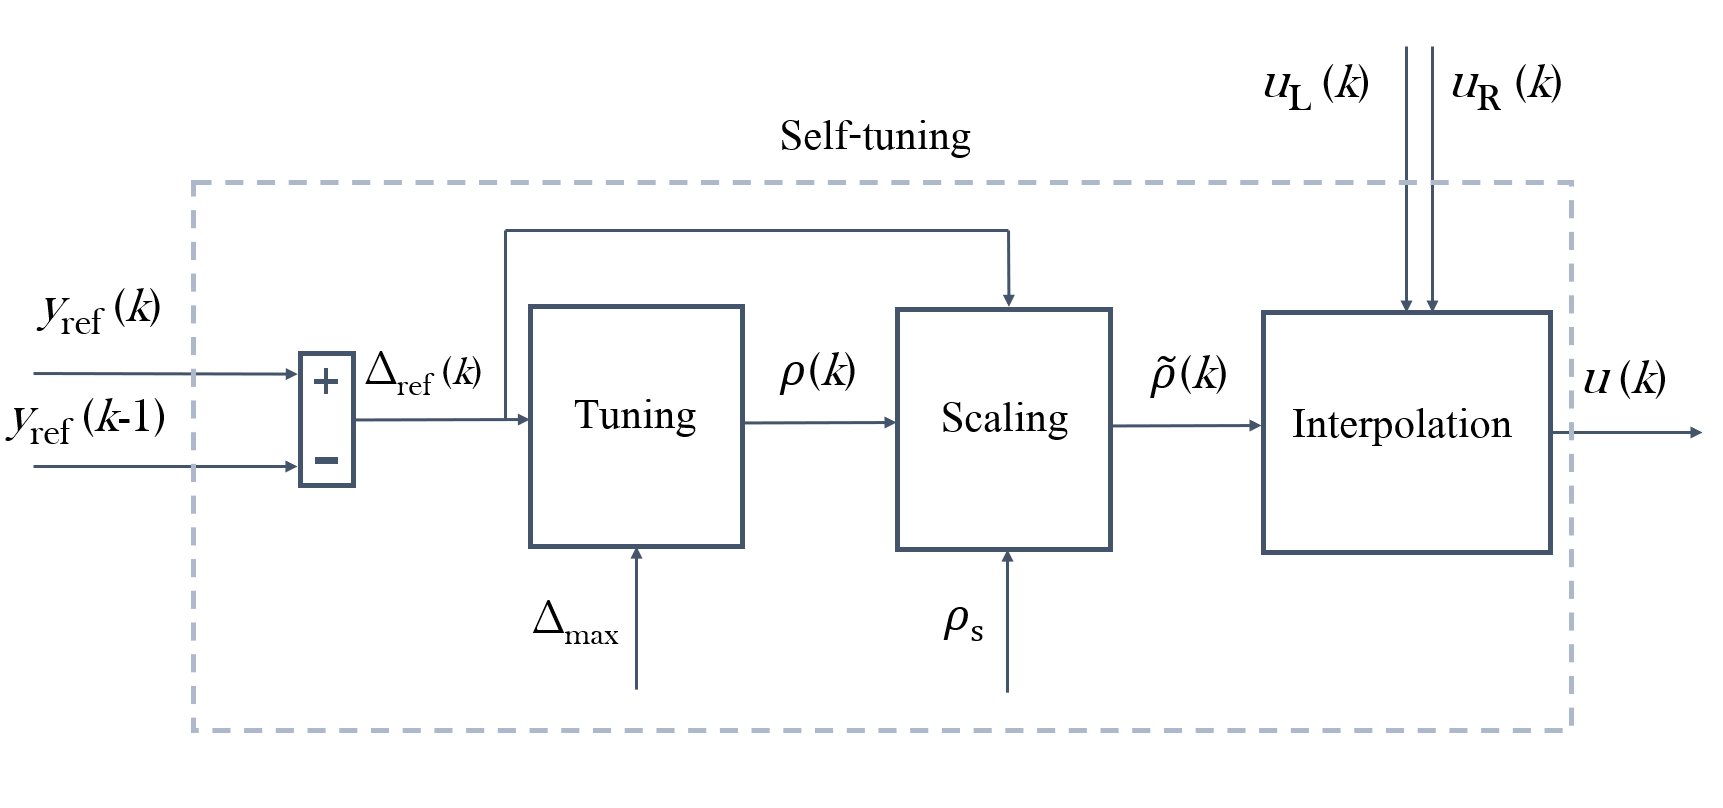
\includegraphics[width=\textwidth]{images/tuning}
		\caption[Self-tuning scheme]{Self-tuning scheme.}
		\label{fig:tuning}
	\end{center}
	\end{figure}

	
	\section{Results and discussion}
\label{sec:results}

In this section, the results of the proposed self-tuning method are analyzed by an experimental implementation. The self-tuning strategy utilizes tuning parameter calculation based on the size of reference change (Section~\ref{sec:self_tunable_delta_ref}) and the scaling of tuning parameter based on splitting the interval of the parameter and assigning the interval parts to specific operating conditions (Section~\ref{sec:self_tunable_rho_scaling}).

The plant on which the control was implemented and analyzed is a laboratory-scaled counter-current liquid-to-liquid plate heat exchanger Armfield Process Plant Trainer PCT23~\cite{pct23}, see Figure~\ref{fig:HE}. The heat exchanger is 90 mm wide, 103 mm long, and 160 mm high. The heat exchange is performed between the cold feed (water) and the hot medium (water). The cold feed as well as the heating medium are transported to the heat exchanger by two peristaltic pumps with flexible tubing from silicon rubber. The flow rate of the feed is constant, while the aim of control is to track the reference value of the feed temperature. Therefore, the controlled variable is the feed temperature $T$ at the outlet of the heat exchanger. The temperature of the heated feed in the outlet stream was measured by the type K thermocouple. The associated manipulated variable is the voltage $U$ corresponding to the power of the pump feeding the heat exchanger by the hot medium. The voltage is within the range of [$0-5$]\,V normalized into the relative values in percentage. For further technical specifications of the laboratory heat exchanger, the reader is referred to~\cite{pct23}. As heat exchange is a nonlinear and asymmetric process~\cite{Liptak}, this heat exchanger represents a suitable candidate for the presented controller tuning strategy. The corresponding simplified closed-loop scheme can be seen in Figure~\ref{fig:CL}. Note, the ,,Self-tuning" block corresponds to the more detailed scheme in Figure~\ref{fig:tuning}.  

The system was identified by experimental identification. More specifically, several step responses were obtained in the whole range of the input variable steps. Every step response was identified as a first-order system and the nominal transfer function was calculated. Finally, the transfer function was converted to the state-space model. The matrices of the discrete-time state-space model of the plant are
\begin{subequations}
	\label{eq:model_A_B} 
	\begin{eqnarray}
		A = \begin{bmatrix}
			0.839
		\end{bmatrix}, \quad
		B = \begin{bmatrix}
			0.039
		\end{bmatrix}, \quad
		C = \begin{bmatrix}
			1
		\end{bmatrix}, 
		%\quad
		%D = \begin{bmatrix}
		%0
		%\end{bmatrix}.
	\end{eqnarray}
\end{subequations}
considering the sampling time $T_\mathrm{s}$ = 1\,s. 
To respect the physical limitations of the operating conditions, the constraints are considered in the terms of control inputs
\begin{eqnarray}
	\label{eq:u_const}
	-15\% \le u \le 65\%,
\end{eqnarray}
where the variable $u$ represents the control inputs in the deviation form. The values of feed temperature and voltage of the heating medium pump corresponding to zero steady states are respectively $T^\mathrm{s}$~=~35 $^{\circ}\mathrm{C}$ and $U^\mathrm{s}$~=~35\%. Therefore, the physical constraints on the manipulated variable are actually
\begin{eqnarray}
	\label{eq:U_const}
	20\% \le U \le 100\%.
\end{eqnarray}	
As the controlled system is naturally stable even if the maximal or minimal value of the manipulated variable is constantly applied, the constraints on the controlled variable in Eq.~\eqref{eq:mpc_problem_state_constraints} can be omitted. Another motivation to include the output/state constraints would be the necessity to retain the controlled variable in some comfort range, specified by operation requirements. As it was not the aim of the case study, this reason also leads to omitting the constraints in Eq.~\eqref{eq:mpc_problem_state_constraints} to fully investigate the control performance of the pure self-tuning method.		 

The penalty matrices of the problem Eq.~\eqref{eq:mpc_problem} were systematically tuned and the corresponding control was implemented on the laboratory heat exchanger for each of the considered explicit MPC setups. 
First, the aim of tuning was to determine, which penalty matrix is the most suitable for real-time tuning. Based on the set of experimentally collected data, the most significant effect on the control trajectories had tuning the penalty matrix $Q_\mathrm{y}$, while still preserving a satisfactory control performance, i.e., without steady-state control error and significant oscillations around the reference value. Next, the boundary values of the tunable matrix $Q_\mathrm{y}$ were tuned as $Q_\mathrm{y, L}$ = 100 and $Q_\mathrm{y, U}$ = 1000. The built-in integrator was penalized with the fixed penalty matrix $Q_\mathrm{x}$ = 1 and the control input with the fixed penalty matrix $R$ = 10. The prediction horizon $N$ was set to 20 control steps. The explicit model predictive controllers were constructed in MATLAB R2020b using the Multi-Parametric Toolbox 3~\cite{mpt_conf}. 

%The initial temperature of the feed was laboratory temperature, i.e., 23$^{\circ}\mathrm{C}$. The temperature of the heating medium was 70$^{\circ}\mathrm{C}$.

The designed explicit model predictive controllers were implemented to track a time-varying PWC reference. 
For the initial 200 seconds, the reference temperature was the steady-state value. After that, the reference changed its value twice upwards and twice downwards. The reference changes also acquired different sizes in order to examine the proposed tuning method as it is dependent on the size of the reference step change. Specifically, the reference temperature values were $T_{\mathrm{ref}}$ = 35$^{\circ}\mathrm{C}$, 45$^{\circ}\mathrm{C}$, 50$^{\circ}\mathrm{C}$, 45$^{\circ}\mathrm{C}$, 35$^{\circ}\mathrm{C}$.

Besides the control design of two boundary explicit MPCs, it was necessary to keep the temperature of the heating medium constant. The heating medium was transported back to the heater after leaving the heat exchanger, i.e., the volume of the heating medium was recycled during the whole operation. The temperature of the heating medium was maintained on the value 70$^{\circ}\mathrm{C}$ with a simple proportional controller with proportional gain $P = 20$. The control input from the proportional controller was the electric power which could acquire the values in the range [$0-2$]\,kW and was also normalized to percentage.

The control profiles generated for both considered boundary control setups are compared in Figure~\ref{fig:CV_boundaries} for the controlled variable, and in Figure~\ref{fig:MV_boundaries} for the control inputs. 
Note, the constructed explicit MPC controller computed control inputs to respect the constraints on the control inputs and they need not be truncated afterward.		

\begin{figure}
	\begin{center}
		\includegraphics[width=0.8\textwidth]{images/HE}
		\caption[Heat exchanger Armfield Process Plant Trainer PCT23]{Laboratory heat exchanger Armfield Process Plant Trainer PCT23: feed pump\,(1), heating medium pump\,(2), feed tanks\,(3), heater for heating medium\,(4), heat exchanger\,(5).}
		\label{fig:HE}
	\end{center}
\end{figure}

\begin{figure}
	\begin{center}
		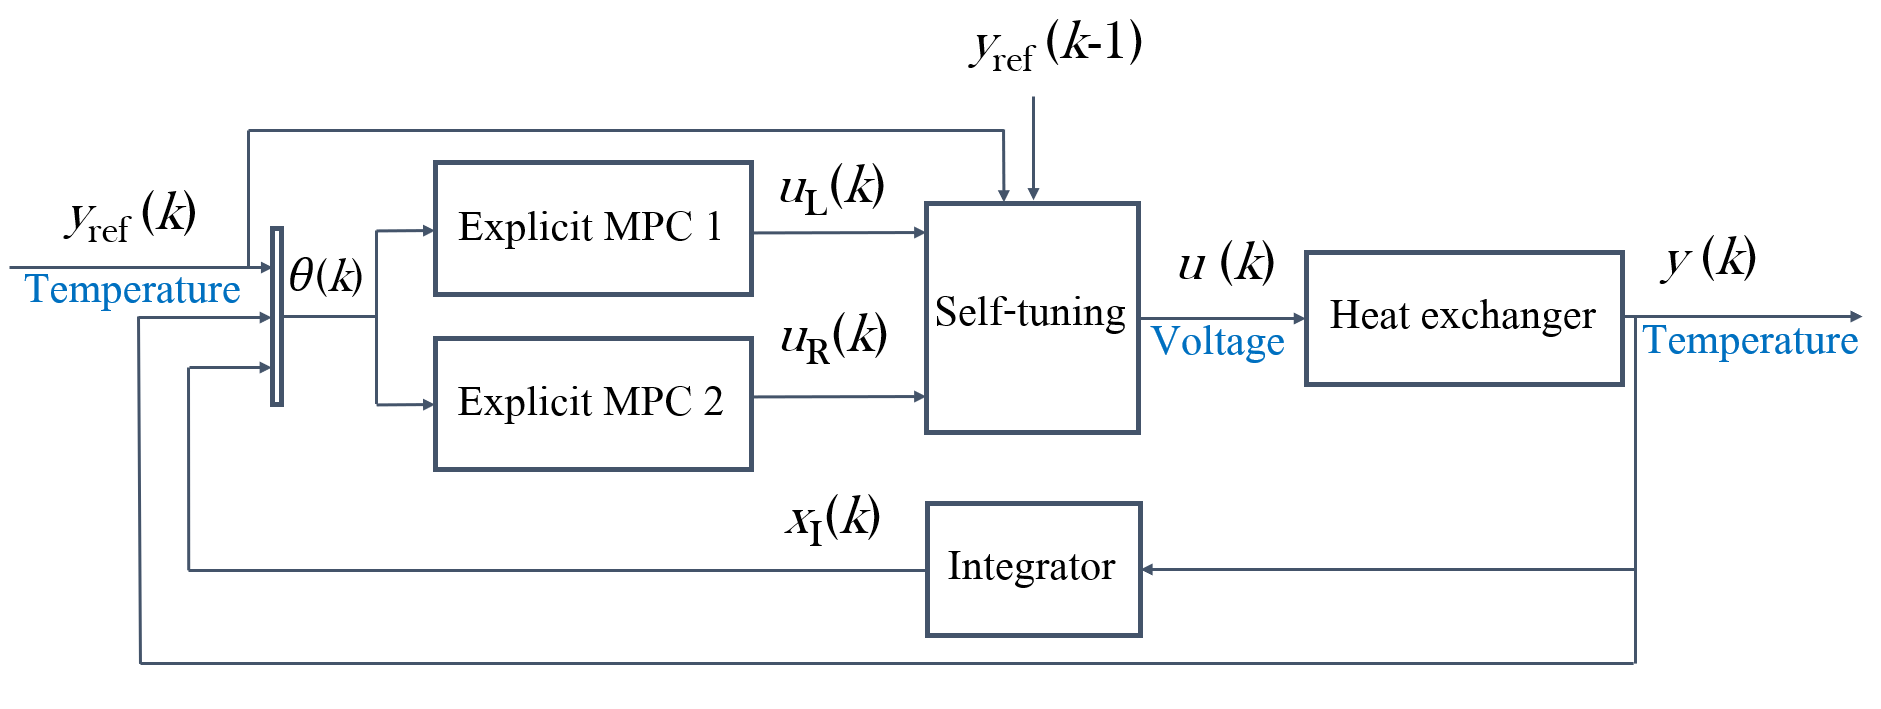
\includegraphics[width=\textwidth]{images/cl}
		\caption[Closed-loop scheme]{Closed-loop scheme.}
		\label{fig:CL}
	\end{center}
\end{figure}

\begin{figure}
	\begin{center}
		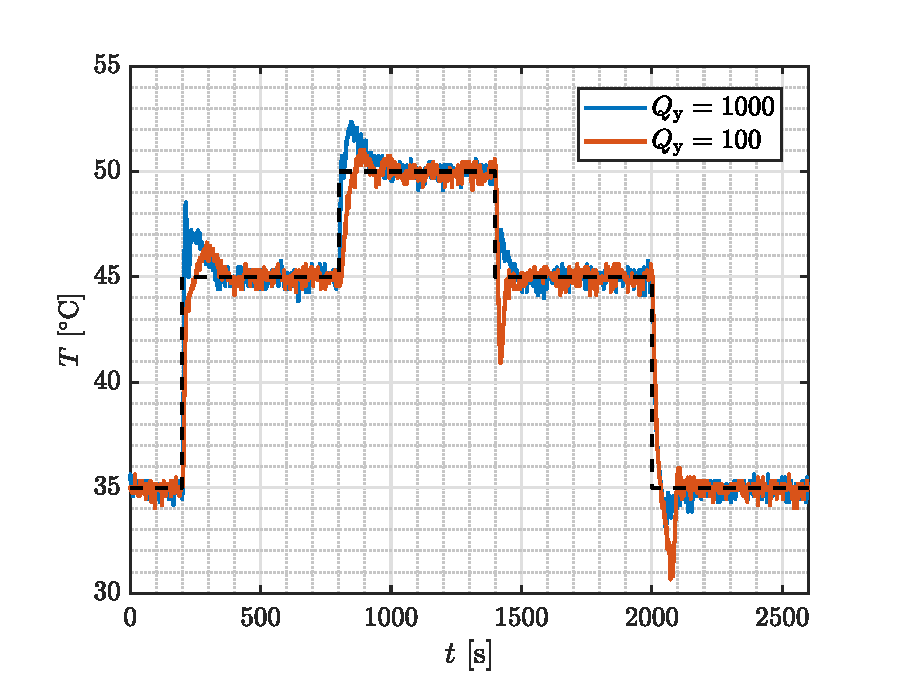
\includegraphics[width=0.8\textwidth]{images/CV_boundaries}
		\caption{Controlled variable trajectory for two boundary controllers. The solid lines represent the controlled temperature $T$ and the dashed line represents the reference value $T_{\mathrm{ref}}$.}
		\label{fig:CV_boundaries}
	\end{center}
\end{figure}

\begin{figure}
	\begin{center}
		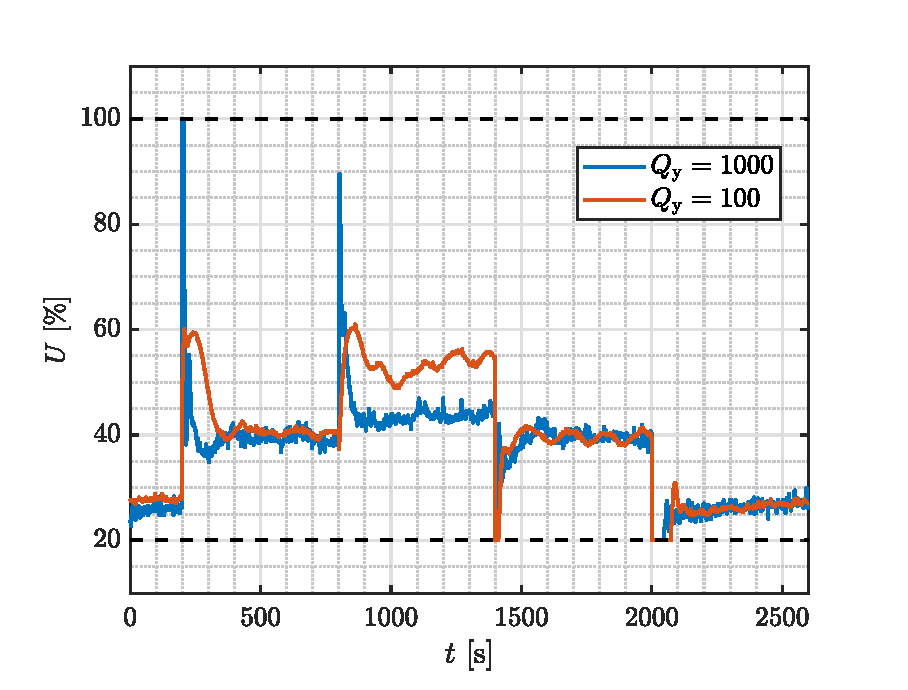
\includegraphics[width=0.8\textwidth]{images/MV_boundaries}
		\caption{Manipulated variable trajectory for two boundary controllers. The solid lines represent the voltage $U$ and the dashed lines represent the constraints.}
		\label{fig:MV_boundaries}
	\end{center}
\end{figure}

The trajectories in Figure~\ref{fig:CV_boundaries} show the asymmetric nature of controlling the plant of plate heat exchange mainly when observing the overshoots and undershoots. When applying the control inputs associated with the lower bound $Q_\mathrm{y, L}$ in Eq.~\eqref{eq:mpc_problem_cost}, significant undershoots are present when tracking the reference downwards, i.e., when the reference change is negative. On the contrary, when implementing the controller associated with $Q_\mathrm{y, U}$ in Eq.~\eqref{eq:mpc_problem_cost}, the undershoots are negligible, but significant overshoots can be seen when tracking the reference upwards.

These main experimental observations established the base for the strategy of self-tuning the penalty matrix $Q_\mathrm{y}$. The strategy follows the ideas summarized in Section~\ref{sec:methodology}. Therefore, utilizing the boundary controller with the penalty matrix $Q_\mathrm{y, L}$ is preferred when the reference changes upwards. On the contrary, the controller associated with $Q_\mathrm{y, U}$ is preferred for negative reference step changes. The splitting value of the tuning parameter was chosen in the middle of the interval, i.e., $\rho_{\mathrm{s}} = 0.5$. The remaining parameter that needed to be set was the maximal admissible size of the reference step change $\Delta_{\max}$, which was determined to $15\,^{\circ}\mathrm{C}$ as the investigated range of controlled temperature was [$35-50$]$^{\circ}\mathrm{C}$. 

The control results of the self-tunable technique compared to the boundary controllers can be seen in Figure~\ref{fig:CV} for the controlled variable, and in Figure~\ref{fig:MV} for the manipulated variable. It can be seen that the tuned controller combined the benefits of the two boundary controllers. The overshoots and undershoots were reduced, as in the first half of control the penalty matrix $Q_\mathrm{y}$ acquired value from the first half of the penalty interval. When tracking the reference with negative step change, the penalty matrix acquired the values from the second half of the interval, i.e., closer to the upper bound $Q_\mathrm{y, U}$. 
The similarity with the boundary controllers can be seen also on the manipulated variable profiles. Note, the constraints on the input variable were satisfied as they were scaled using linear interpolation based on the boundary controllers which are constructed considering the input constraints. 

\begin{figure}
	\begin{center}
		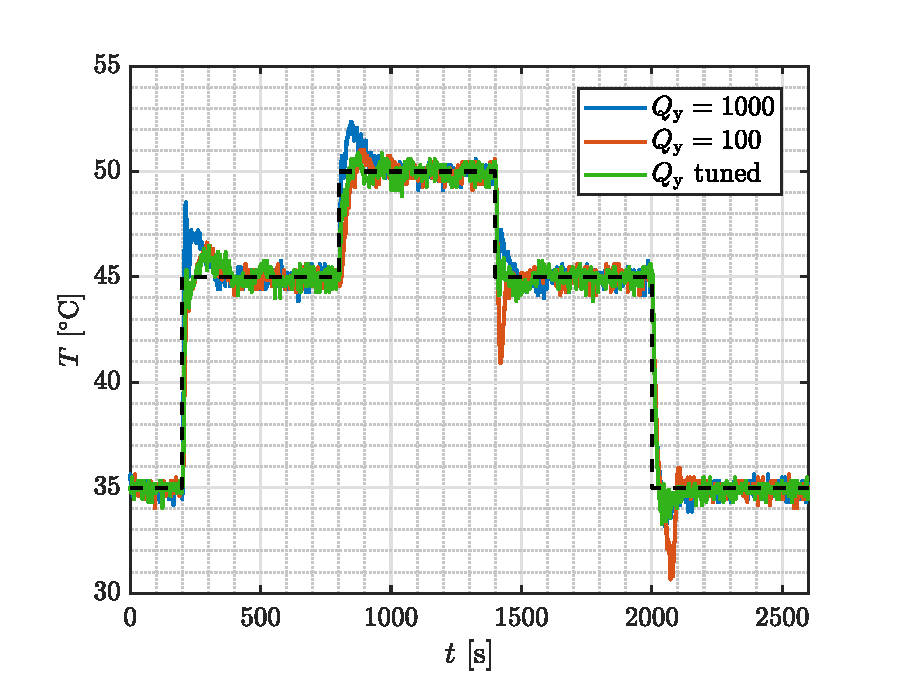
\includegraphics[width=0.8\textwidth]{images/CV}
		\caption{Controlled variable trajectory for two boundary controllers and the tuned one. The solid lines represent the controlled temperature $T$ and the dashed line represents the reference value $^{\circ}\mathrm{C}$.}
		\label{fig:CV}
	\end{center}
\end{figure}

\begin{figure}
	\begin{center}
		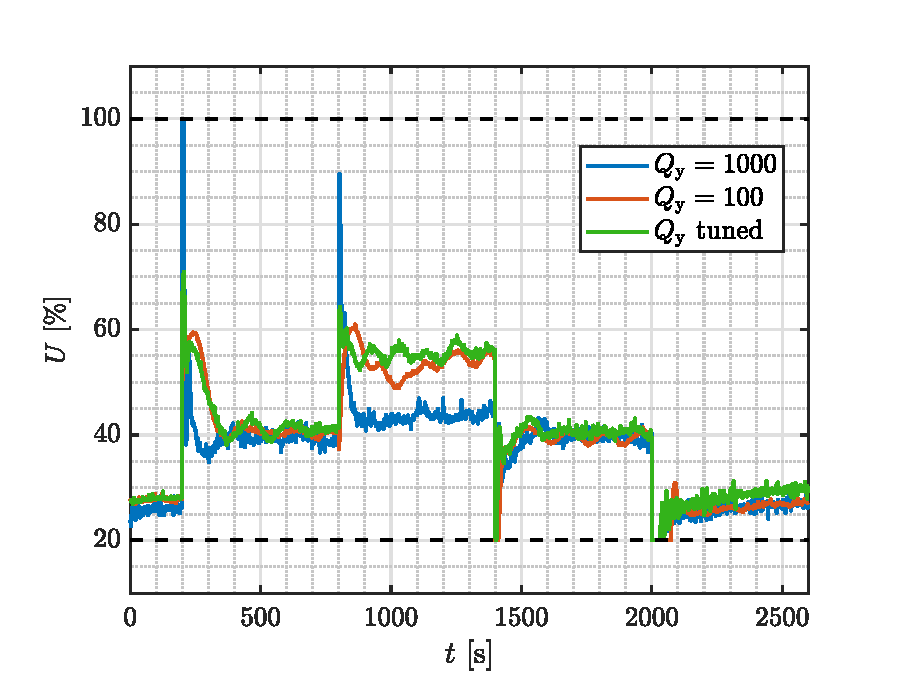
\includegraphics[width=0.8\textwidth]{images/MV}
		\caption{Manipulated variable trajectory for two boundary controllers and the tuned one. The solid lines represent the voltage $U$ and the dashed lines represent the constraints.}
		\label{fig:MV}
	\end{center}
\end{figure}

The control performance was also investigated quantitatively. Table~\ref{tab:control_performance} summarizes the evaluated control performance criteria computed for the two boundary controllers and the self-tuned controller. The control performance is evaluated for each reference step change separately. The considered quality criteria are: sum-of-squared based criterion -- integral squared error $ISE$, maximal overshoot/undershoot $\sigma_{\mathrm{max}}$ and the settling time $t_{\epsilon}$ for 5\,\%-neighbourhood of the reference temperature $T_{\mathrm{ref}}$. To provide better readability of the computed results in Table~\ref{tab:control_performance}, the best values, i.e., the minimum values, are emphasized using a bold font style. 

%	\begin{table}[h!]
%		\begin{center}
%			\caption{Control performance criteria.}
%			\label{tab:control_performance}
%			\begin{tabular}{c|c|c|c|c|c} 
%				Reference step change & $Q_\mathrm{y}$ & $ISE$ [$^{\circ}\mathrm{C}^2$\,s] & $\sigma_{\mathrm{max}}$\,[\%] & $t_{\epsilon}$\,[s] & $V$\,[l] \\
%				\hline
%				\multirow{2}{*}{ 35\,$^{\circ}$C $\rightarrow$ 45\,$^{\circ}$C } & 1000 & 714 & 33.50 & 16.5 & \textbf{2.12} \\
%				& 100 & 867 & 16.65 & 12.5 & 2.36 \\ 
%				& self-tuned & \textbf{678} & \textbf{15.19} & \textbf{9.5} & 2.38 \\ 
%				\hline
%				\multirow{2}{*}{ 45\,$^{\circ}$C $\rightarrow$ 50\,$^{\circ}$C } & 1000 & 365 & 47.20 & \textbf{5} & \textbf{2.49} \\
%				& 100 & 606 & 23.25 & 26.5 & 3.19 \\ 
%				& self-tuned & \textbf{248} & \textbf{19.13} & 9.5 & 3.35 \\ 
%				\hline
%				\multirow{2}{*}{ 50\,$^{\circ}$C $\rightarrow$ 45\,$^{\circ}$C } & 1000 & 245 & \textbf{18.92} & \textbf{6.5} & \textbf{2.00} \\
%				& 100 & 398 & 79.64 & 31 & \textbf{2.00} \\ 
%				& self-tuned & \textbf{186} & 24.59 & \textbf{6.5} & 2.10 \\ 
%				\hline
%				\multirow{2}{*}{ 45\,$^{\circ}$C $\rightarrow$ 35\,$^{\circ}$C } & 1000 & 1024 & 18.43 & 22.5 & 0.94 \\
%				& 100 & 1402 & 41.87 & 90 & \textbf{0.93} \\ 
%				& self-tuned & \textbf{967} & \textbf{16.49} & \textbf{18.5} & 1.10  
%			\end{tabular}
%		\end{center}
%	\end{table}

\begin{table}[h!]
	\begin{center}
		\caption{Control performance criteria.}
		\label{tab:control_performance}
		\begin{tabular}{c|c|c|c|c} 
			Reference step change & $Q_\mathrm{y}$ & $ISE$ [$^{\circ}\mathrm{C}^2$\,s] & $\sigma_{\mathrm{max}}$\,[\%] & $t_{\epsilon}$\,[s]  \\
			\hline
			\multirow{2}{*}{ 35\,$^{\circ}$C $\rightarrow$ 45\,$^{\circ}$C } & 1000 & 714 & 33.50 & 16.5 \\
			& 100 & 867 & 16.65 & 12.5 \\ 
			& self-tuned & \textbf{678} & \textbf{15.19} & \textbf{9.5}  \\ 
			\hline
			\multirow{2}{*}{ 45\,$^{\circ}$C $\rightarrow$ 50\,$^{\circ}$C } & 1000 & 365 & 47.20 & \textbf{5} \\
			& 100 & 606 & 23.25 & 26.5  \\ 
			& self-tuned & \textbf{248} & \textbf{19.13} & 9.5  \\ 
			\hline
			\multirow{2}{*}{ 50\,$^{\circ}$C $\rightarrow$ 45\,$^{\circ}$C } & 1000 & 245 & \textbf{18.92} & \textbf{6.5}  \\
			& 100 & 398 & 79.64 & 31  \\ 
			& self-tuned & \textbf{186} & 24.59 & \textbf{6.5}  \\ 
			\hline
			\multirow{2}{*}{ 45\,$^{\circ}$C $\rightarrow$ 35\,$^{\circ}$C } & 1000 & 1024 & 18.43 & 22.5  \\
			& 100 & 1402 & 41.87 & 90  \\ 
			& self-tuned & \textbf{967} & \textbf{16.49} & \textbf{18.5}   
		\end{tabular}
	\end{center}
\end{table}

As can be seen in Table~\ref{tab:control_performance}, the real-time self-tuning of the explicit MPC controller helped to improve two to three criteria when tracking each reference value. 	
The relative improvement in the percentage, denoted by $\delta$, of using the self-tunable controller computed subject to the second best setup is summarized in Table~\ref{tab:improvement} for each reference step change separately. The negative numbers represent deterioration compared to the best controller setup in the corresponding reference tracking. 

\begin{table}[h!]
	\begin{center}
		\caption{Relative improvement of the control performance using the self-tunable explicit MPC controller.}
		\label{tab:improvement}
		\begin{tabular}{c|c|c|c} 
			Reference step change & $\delta ISE$\,[\%] & $\delta \sigma_{\mathrm{max}}$\,[\%] & $\delta t_{\epsilon}$\,[\%]  \\
			\hline
			35\,$^{\circ}$C $\rightarrow$ 45\,$^{\circ}$C &  5 &  9 & 24 \\ 
			% \hline
			45\,$^{\circ}$C $\rightarrow$ 50\,$^{\circ}$C & 32 & 18 &$-90$  \\ 
			% \hline
			50\,$^{\circ}$C $\rightarrow$ 45\,$^{\circ}$C & 24 &$-30$& 0 \\ 
			% \hline
			45\,$^{\circ}$C $\rightarrow$ 35\,$^{\circ}$C &  6 & 11 & 18   
		\end{tabular}
	\end{center}
\end{table}
%\begin{table}[h!]
%\begin{center}
%\caption{Relative improvement of the control performance using the self-tunable explicit MPC controller.}
%\label{tab:improvement}
%\begin{tabular}{c|c|c|c|c} 
%Reference step change & $\Delta ISE$\,[\%] & $\Delta \sigma_{\mathrm{max}}$\,[\%] & $\Delta t_{\epsilon}$\,[\%] & $\Delta V$\,[\%] \\
%\hline
%35\,$^{\circ}$C $\rightarrow$ 45\,$^{\circ}$C & 5.04 & 8.77 & 24.00 & -12.26 \\ 
%\hline
%45\,$^{\circ}$C $\rightarrow$ 50\,$^{\circ}$C & 32.05 & 17.72 & -90.00 & -34.54 \\ 
%\hline
%45\,$^{\circ}$C $\rightarrow$ 50\,$^{\circ}$C & 24.08 & -29.97 & 0 & -4.48 \\ 
%\hline
%45\,$^{\circ}$C $\rightarrow$ 35\,$^{\circ}$C & 5.57 & 10.53 & 17.78 & -18.28  
%\end{tabular}
%\end{center}
%\end{table}


Compared to the considered non-self-tunable controllers, the control trajectories and the evaluated quality criteria confirmed the improved control performance for the reference tracking control problem of the heat exchanger with the non-linear and asymmetric behavior. Implementing a self-tunable explicit MPC controller leads to improved control performance in the most analyzed quality criteria, see Table~\ref{tab:improvement}.	 
The squared-error-based criterion ($ISE$) improved in every control scenario within a range $[5-32]$\,\%, the maximal overshoots/undershoots $\sigma_{\mathrm{max}}$ reduced up to 18\,\%, and the settling time $t_{\epsilon}$ decreased up to 24\,\%.  

To analyze the control more objectively, energy consumption was also investigated. More specifically, the power used to heat the heating medium was measured and summarized for the whole control but for every controller setup, respectively. The energy consumption $E$ necessary for every control can be seen in Table~\ref{tab:energy}.

\begin{table}[h!]
	\begin{center}
		\caption{Energy consumption evaluation.}
		\label{tab:energy}
		\begin{tabular}{c|c} 
			$Q_\mathrm{y}$ & E\,[kJ]   \\
			\hline
			1000 &  883  \\ 
			% \hline
			100 & 938   \\ 
			% \hline
			self-tuned & 921   
		\end{tabular}
	\end{center}
\end{table}

It can be seen in Table~\ref{tab:energy}, that utilizing the self-tuned controller leads to energy consumption which acquires value between the energy consumptions associated with the boundary controllers. Although it is not the minimum one, the energy is still saved compared to the boundary controller with $Q_\mathrm{y} = 100$. Note, though the controller with $Q_\mathrm{y} = 1000$ leads to minimum energy consumption, using this single non-tuned controller does not lead to such control performance improvement.

In general, utilizing the proposed controller with a scalable aggressiveness according to the operating conditions leads to higher accuracy (lower $ISE$), lower value of the overshoots (lower $\sigma_{\mathrm{max}}$), and faster achieving the reference value (lower $t_{\epsilon}$), while the control does not suffer in the terms of energy consumption. 



%	Together with the reduced overshoots and settling times, the achieved improvements in the control performance enable non-negligible energy savings when the precision and the operating time ensure the product with the required properties.  

\section{Conclusions}
\label{sec:conclusion}

	This paper deals with the experimental implementation of the self-tunable approximated explicit model predictive control and provides a strategy for an effective self-tuning controller design. Based on the current reference value, the tuning parameter is scaled using linear interpolation. The previously published work related to the self-tunable explicit MPC suggested tuning based on the distance of the reference value from the system steady-state value. This paper presents a novel idea of tuning based on the size of reference step change. The self-tuning algorithm aims to compensate for the nonlinear behavior of the controlled system. The self-tuning parameter is updated when the reference changes. It is calculated as the ratio between the size of the reference change and the maximal possible size of the reference change, which is specified before operation. 
	Another novel contribution addresses the challenging control problem of asymmetric system behavior by splitting the interval of tuning parameter into two ranges, while both intervals are assigned to different operating conditions. The proposed method is implemented on a laboratory heat exchanger with nonlinear and asymmetric behavior. The asymmetry makes the plant a suitable candidate for splitting the interval of the tuning parameter. The decision criterium is negativity or positivity of reference change. When the reference changed upwards, the control input was tuned in the first part of the interval and approached the boundary controller associated with the lower bound on the penalty matrix. On the contrary, when the reference changed downwards, the control input was tuned to approach the control input from the boundary controller with the upper bound on the penalty matrix. To investigate the control results properly, the control performance was evaluated also quantitatively. Compared to the conventional control strategy handling just a single controller, the self-tunable control approach decreased the integral squared control error, maximal overshoots/undershoots, and settling time. In addition, the energy consumption corresponding to every controller was evaluated as well. The value of consumed energy was between the two boundary controllers, i.e., the energy consumption did not deteriorate in general. With saving energy compared to one of the boundary controllers, the control performance was significantly improved. 
	
	\section*{Acknowledgments}
	
	The authors gratefully acknowledge the contribution of the Scientific Grant Agency of the Slovak Republic under the grants 1/0545/20, 1/0297/22, and the Slovak Research and Development Agency under the project APVV-20-0261. 
	This research is funded by the European Union’s Horizon Europe under grant no. 101079342 (Fostering Opportunities Towards Slovak Excellence in Advanced Control for Smart Industries). 
	
	\section*{Nomenclature}
	
	\subsection*{Symbols}
%	\begin{center}
		\begin{tabular}{ l l }
			$A$ & system state matrix \\
			$\widetilde{A}$ & augmented system state matrix \\
			$B$ & system input matrix \\
			$\widetilde{B}$ & augmented system input matrix \\
			$C$ & system output matrix \\
			$\widetilde{C}$ & augmented system output matrix \\
			$d_{\max}$ & maximal deviation from the steady-state value \\
			$F$ & slope of the affine control law \\
			$g$ & section of the affine control law \\
			$I$ & identity matrix \\
			$k$ & step of the prediction horizon \\
			$N$ & prediction horizon \\
			$n_{\mathrm{u}}$ & size of system inputs \\
			$n_{\mathrm{y}}$ & size of system outputs \\
			$n_{\widetilde{\mathrm{x}}}$ & size of augmented system states \\
			$P$ & proportional gain of proportional controller\\
			$Q_{\mathrm{x}}$ & penalty matrix of the built-in integrator \\
			$Q_{\mathrm{x,L}}$ & lower bound on the penalty matrix of the built-in integrator \\
			$Q_{\mathrm{x,U}}$ & upper bound on the penalty matrix of the built-in integrator \\
			$Q_{\mathrm{y}}$ & penalty matrix of the control error \\
			$Q_{\mathrm{y,L}}$ & lower bound on the penalty matrix of the control error \\
			$Q_{\mathrm{y,U}}$ & upper bound on the penalty matrix of the control error \\
			$R$ & penalty matrix of system inputs \\
			$R_{\mathrm{L}}$ & lower bound on the penalty matrix of system inputs \\
			$R_{\mathrm{U}}$ & upper bound on the penalty matrix of system inputs \\
			$\mathcal{R}$ & critical region \\
			$\mathbb{R}$ & Euclidean space of real numbers \\
			$t$ & time, s \\
			$t_{\epsilon}$ & settling time, s \\
			$T$ & temperature, $^{\circ}\mathrm{C}$ \\
			$T_{\mathrm{ref}}$ & reference temperature, $^{\circ}\mathrm{C}$ \\
			$T_{\mathrm{s}}$ & sampling time, s \\
			$T^{\mathrm{s}}$ & steady state of temperature, $^{\circ}\mathrm{C}$ \\
			$u$ & control inputs \\
		\end{tabular}
%	\end{center}
	
	%% Page - break
	
%	\begin{center}
		\begin{tabular}{ l l }
			$u_{\mathrm{L}}$ & control inputs associated with the lower boundary controller\\
			$u_{\mathrm{U}}$ & control inputs associated with the upper boundary controller\\
			$U$ & voltage, \% \\
			$U^{\mathrm{s}}$ & steady state of voltage, \% \\
			$\mathcal{U}$ & set of control inputs \\			
			$x$ & system states \\
			$\widetilde{x}$ & augmented system states \\
			$x_{\mathrm{I}}$ & system states corresponding to the built-in integrator \\
			$y$ & system outputs \\
			$y_\mathrm{\max}$ & maximal value of system outputs \\
			$y_\mathrm{\min}$ & minimal value of system outputs \\
			$y_\mathrm{ref}$ & reference value of system outputs \\
			$\mathcal{Y}$ & set of system outputs \\
			\textit{0} & zero matrix
		\end{tabular}
%	\end{center}
	
	\subsection{Greek letters}
%	\begin{center}
		\begin{tabular}{ l l }
			$\delta$ & relative improvement, \% \\
			$\Delta_\mathrm{max}$ & maximal size of the reference change, $^{\circ}\mathrm{C}$  \\
			$\Delta_\mathrm{ref}$ & size of the reference change, $^{\circ}\mathrm{C}$ \\
			$\rho$ & tuning factor \\
			$\widetilde{\rho}$ & scaled tuning factor \\
			$\rho_{\mathrm{s}}$ & splitting value of the tuning factor \\
			$\sigma_{\max}$ & maximal overshoot, \% \\
			$\theta$ & parameter of optimization problem \\
			$\Theta$ & set of parameter values
		\end{tabular}
%	\end{center}
	
	\subsection*{Abbreviations}
%	\begin{center}
		\begin{tabular}{ l l }
			ISE  & integral squared error \\
			LTI  & linear time-invariant (system) \\
			MIMO & multiple-inputs and multiple-outputs (system) \\
			MPC  & model predictive control \\
			mp-QP& multi-parametric quadratic programming (problem) \\
			PID  & proportional–integral–derivative (controller) \\
			PWA  & piece-wise affine (function) \\
			PWC  & piece-wise constant (function) \\
			QP   & quadratic programming (problem) \\
			SISO & single-input and single-output (system) \\
		\end{tabular}
%	\end{center}
	
	%% The Appendices part is started with the command \appendix;
	%% appendix sections are then done as normal sections
	%% \appendix
	
	%% \section{}
	%% \label{}
	
	%% If you have bibdatabase file and want bibtex to generate the
	%% bibitems, please use
	%%
	
	\bibliographystyle{elsarticle-num} 
	\bibliography{references}
	
	%% else use the following coding to input the bibitems directly in the
	%% TeX file.
	
	%\begin{thebibliography}{00}
		%
		%%% \bibitem{label}
		%%% Text of bibliographic item
		%
		%\bibitem{}
		%
		%\end{thebibliography}
	
\end{document}
\endinput
%%
%% End of file `elsarticle-template-num.tex'.